\chapter{От граничных условий к спектру открытой струны}

\lectureoverview{Наша цель — квантовать открытую струну и решить, заслуживают ли её состояния того, чтобы называться частицами. Путь будет элементарным, но требовательным. Сначала мы подготовим аппарат анализа и разложения Фурье для функций на \(0\leq\sigma\leq\pi\). Затем мы заменим точечность спектральным критерием поведения частицы, рассмотрим описание при бесконечном импульсе, в котором поперечная динамика становится нерелятивистской, и построим струну из цепочки лёгких масс и жёстких пружин. Непрерывная струна — это волновая система со свободными концами. Её моды Неймана распадаются на гармонические осцилляторы с частотами \(1,2,3,\ldots\); поэтому квантование приводит к дискретному спектру с щелью. Наконец, взаимодействия струн вынуждают нас выйти за пределы открытых струн: открытая струна может соединить свои собственные концы и стать замкнутой.}

\section{Математический анализ на отрезке открытой струны}

В вычислениях нам неоднократно придётся заменять дискретные суммы интегралами, а разности между соседними элементами — производными. Лучше заранее зафиксировать эти факты, прежде чем они будут прерывать физическое обсуждение.

Пусть \(x(\sigma)\) — функция на

\begin{equation}
  0\leq \sigma\leq \pi .
\end{equation}

Обозначения выбраны с прицелом на теорию струн: \(\sigma\) обозначает положение вдоль струны, тогда как \(x\) станет одной из её поперечных координат. Разобьём интервал на \(N\) частей,

\begin{equation}
  \Delta\sigma=\frac{\pi}{N},
  \qquad
  \sigma_i=i\,\Delta\sigma,
  \qquad
  x_i=x(\sigma_i).
  \label{eq:l02-lattice}
\end{equation}

Для гладкой предельной функции,

\begin{equation}
  \Delta x_i\equiv x_i-x_{i-1}
  =
  \frac{\partial x}{\partial\sigma}\,\Delta\sigma
  +O\!\left((\Delta\sigma)^2\right),
  \label{eq:l02-difference}
\end{equation}

а сумма Римана переходит в

\begin{equation}
  \sum_i x_i\,\Delta\sigma
  \longrightarrow
  \int_0^\pi x(\sigma)\,d\sigma .
  \label{eq:l02-riemann}
\end{equation}

\begin{figure}[H]
  \centering
  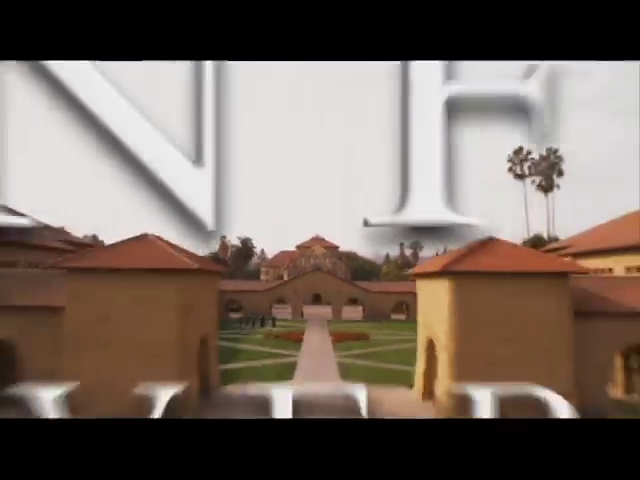
\includegraphics[width=0.78\textwidth]{lecture_02_figure_01.png}
  \caption{Правила для конечных разностей и сумм Римана, оставленные на доске для последующего перехода к непрерывному пределу.}
  \lectureframe{00:04:20}
  \label{fig:l02-calculus-board}
\end{figure}

Это определения, знакомые из математического анализа. Здесь важно их масштабирование: \(\Delta x_i\) даёт одну степень \(\Delta\sigma\), тогда как сумма при переходе в интеграл даёт одну обратную степень.

\subsection{Граничные условия Дирихле и Неймана}

Разложение Фурье на конечном интервале начинается с выбора граничных условий на концах. Нам будут снова встречаться два варианта.

\begin{align}
  \text{Dirichlet:}\qquad
  &x(0)=x(\pi)=0,
  \label{eq:l02-dirichlet}\\
  \text{Neumann:}\qquad
  &\left.\partial_\sigma x\right|_{\sigma=0}
   =
   \left.\partial_\sigma x\right|_{\sigma=\pi}
   =0.
  \label{eq:l02-neumann}
\end{align}

Скрипичная струна, закреплённая на обоих концах, иллюстрирует случай Дирихле: её смещение обращается в нуль на границах. Функция Неймана не обязана там обращаться в нуль; у каждой границы её наклон равен нулю. Обе характерные формы вместе показаны на доске.

\begin{figure}[H]
  \centering
  \begin{minipage}[t]{0.48\textwidth}
    \centering
    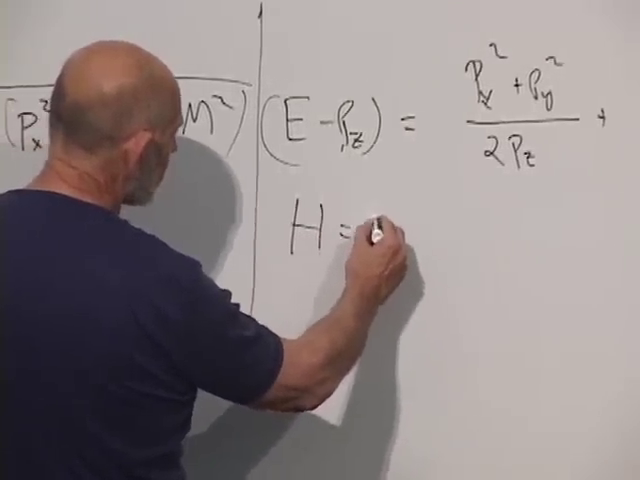
\includegraphics[width=\textwidth]{lecture_02_figure_02.png}
    \par\smallskip\footnotesize (a) Профили с закреплёнными и горизонтальными концами.
  \end{minipage}\hfill
  \begin{minipage}[t]{0.48\textwidth}
    \centering
    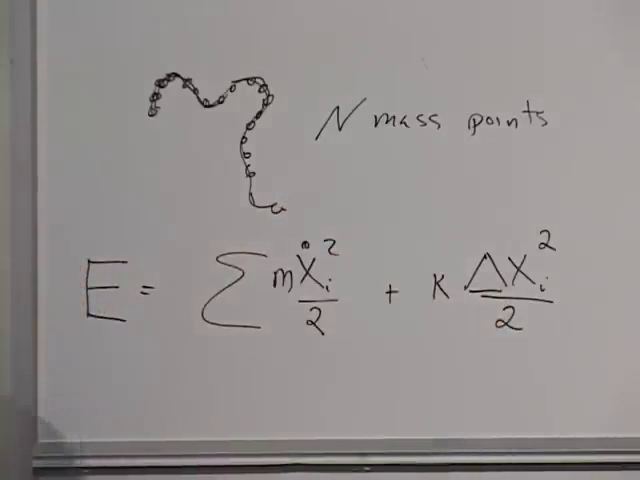
\includegraphics[width=\textwidth]{lecture_02_figure_03.png}
    \par\smallskip\footnotesize (b) Лёгкие кольца, скользящие по вертикальным стержням.
  \end{minipage}
  \caption{Граничные условия как формы и как механика. Конструкция со скользящими кольцами задаёт свободному концу однозначно определённое поперечное движение.}
  \lectureframe{00:08:50 and 00:12:15}
  \label{fig:l02-boundaries-board}
\end{figure}

\begin{figure}[H]
  \centering
  \begin{adjustbox}{max width=\linewidth}
  \begin{tikzpicture}[>=Latex,thick,scale=0.92]
    \begin{scope}
      \draw[->] (0,0) -- (4.4,0) node[right] {\(\sigma\)};
      \draw[->] (0,-1.25) -- (0,1.35) node[above] {\(x\)};
      \draw[blue!70!black]
        (0,0) .. controls (0.8,1.1) and (1.4,1.0) .. (2.0,0)
        .. controls (2.7,-1.0) and (3.4,-0.8) .. (4.1,0);
      \fill (0,0) circle (0.06);
      \fill (4.1,0) circle (0.06);
      \node at (2.05,-1.65) {Dirichlet: \(x=0\)};
    \end{scope}
    \begin{scope}[xshift=5.8cm]
      \draw[->] (0,0) -- (4.4,0) node[right] {\(\sigma\)};
      \draw[->] (0,-1.25) -- (0,1.35) node[above] {\(x\)};
      \draw[orange!85!black]
        (0,0.65) .. controls (0.8,0.65) and (1.1,-0.9) .. (2.0,-0.9)
        .. controls (2.9,-0.9) and (3.2,0.55) .. (4.1,0.55);
      \draw[orange!85!black] (0,0.65) -- (0.45,0.65);
      \draw[orange!85!black] (3.65,0.55) -- (4.1,0.55);
      \node at (2.05,-1.65) {Neumann: \(\partial_\sigma x=0\)};
    \end{scope}
  \end{tikzpicture}
  \end{adjustbox}
  \caption{При данных Дирихле фиксируется значение; при данных Неймана — наклон.}
  \label{fig:l02-boundaries-redraw}
\end{figure}

\begin{classroomqa}
\audiencequestion{Даёт ли открытая или закрытая органная труба чистый пример одного из этих граничных условий?\lecturetimestamp{00:09:19}}
\lecturerresponse{Может, но сначала нужно сказать, по какой акустической переменной ведётся разложение. Возмущение давления и продольное смещение подчиняются на открытом конце взаимно дополнительным идеализированным условиям. Вместо того чтобы разбирать этот побочный вопрос у доски, воспользуемся моделью со скользящими кольцами: почти безмассовые кольца могут двигаться вертикально вдоль стержней, поэтому концы струны свободны и картина Неймана реализуется непосредственно.}
\end{classroomqa}

\begin{classroomqa}
\audiencequestion{Может ли график подниматься вертикально и содержать резкий скачок?\lecturetimestamp{00:09:53}}
\lecturerresponse{Разложение Фурье допускает изолированные скачки у кусочно-непрерывной функции. Для физической струны ограничения строже. Скачок разъединяет соседние точки и делает пространственную производную \(\partial_\sigma x\) сингулярной в непрерывной энергии, которую мы выведем ниже. Поэтому мы ограничимся профилями, которые непрерывны и дифференцируемы.}
\end{classroomqa}

\begin{classroomqa}
\audiencequestion{Почему открытый конец трубы, или вообще любой свободный конец, должен вообще удовлетворять какому-то граничному условию?\lecturetimestamp{00:11:14}}
\lecturerresponse{Акустический пример зависит от выбранного поля и в обсуждении остался неразрешённым. Механический пример — нет. Очень лёгкое кольцо свободно скользит, но всё же прикреплено к последнему участку струны. Мы выведем соответствующее условие из закона Ньютона, а не будем просто постулировать его: конечное ускорение конца вынуждает наклон обращаться в нуль.}
\end{classroomqa}

\subsection{Базисы Фурье}

Как только класс граничных условий на концах выбран, соответствующий базис Фурье тем самым определён. На \(0\leq\sigma\leq\pi\),

\begin{align}
  x_D(\sigma)
  &=
  \sum_{n=1}^{\infty}x_n\sin(n\sigma),
  \label{eq:l02-dirichlet-series}\\
  x_N(\sigma)
  &=
  \sum_{n=0}^{\infty}x_n\cos(n\sigma).
  \label{eq:l02-neumann-series}
\end{align}

Каждый синус в \eqref{eq:l02-dirichlet-series} обращается в нуль на обоих концах. У каждого косинуса в \eqref{eq:l02-neumann-series} производная на концах равна нулю. Нижние пределы различаются не случайно: \(\sin(0\sigma)=0\) ничего не даёт, тогда как \(\cos(0\sigma)=1\) — это постоянная, или нулевая, мода. Она задаёт среднее значение функции Неймана.

\begin{figure}[H]
  \centering
  \begin{minipage}[t]{0.48\textwidth}
    \centering
    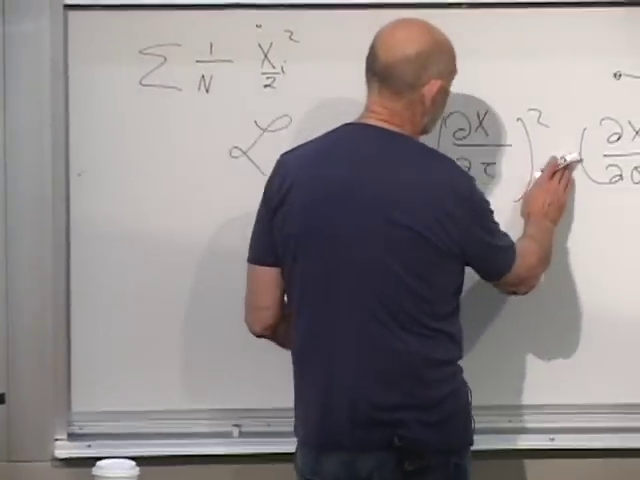
\includegraphics[width=\textwidth]{lecture_02_figure_04.png}
    \par\smallskip\footnotesize (a) Разложения по синусам и косинусам.
  \end{minipage}\hfill
  \begin{minipage}[t]{0.48\textwidth}
    \centering
    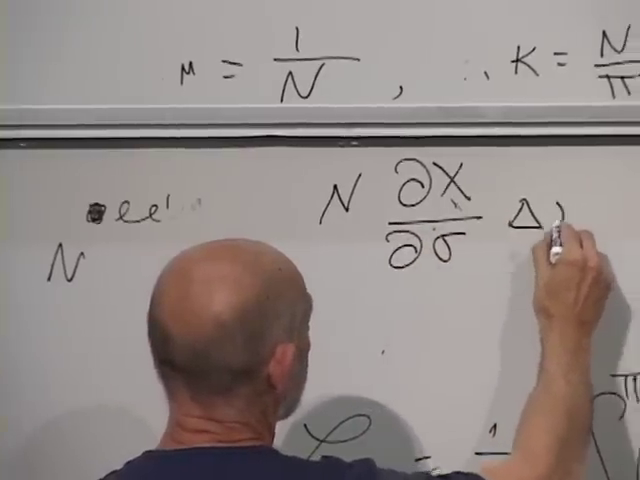
\includegraphics[width=\textwidth]{lecture_02_figure_05.png}
    \par\smallskip\footnotesize (b) Ортогональность и особая постоянная мода.
  \end{minipage}
  \caption{Факты о разложении Фурье, которые далее будут использованы для диагонализации струны.}
  \lectureframe{00:16:15 and 00:20:30}
  \label{fig:l02-fourier-board}
\end{figure}

Дифференцирование переводит один класс в другой:

\begin{equation}
  \begin{aligned}
    \partial_\sigma\sin(n\sigma)&=n\cos(n\sigma),\\
    \partial_\sigma\cos(n\sigma)&=-n\sin(n\sigma).
  \end{aligned}
  \label{eq:l02-basis-derivatives}
\end{equation}

Поэтому производная ряда Дирихле имеет поведение Неймана, а производная ряда Неймана — поведение Дирихле. Ортогональность затем устраняет перекрёстные члены между различными модами:

\begin{align}
  \int_0^\pi\cos(n\sigma)\cos(m\sigma)\,d\sigma
  &=
  \frac{\pi}{2}\delta_{nm},
  && n,m\geq1,
  \label{eq:l02-cos-orthogonality}\\
  \int_0^\pi\sin(n\sigma)\sin(m\sigma)\,d\sigma
  &=
  \frac{\pi}{2}\delta_{nm},
  && n,m\geq1,
  \label{eq:l02-sin-orthogonality}\\
  \int_0^\pi 1\,d\sigma&=\pi .
  \label{eq:l02-zero-norm}
\end{align}

Последняя строка — это особая норма косинуса при \(n=m=0\). Постоянная нормируется не так, как ненулевая гармоника, и этот множитель 2 будет отличать моду центра масс струны от её внутренних мод.

\subsection{Одна формула для осциллятора, которую стоит запомнить}

После перенормировки координаты так, чтобы её механическая масса была равна единице, для осциллятора с законом Гука имеем

\begin{align}
  E_{\mathrm{osc}}
  &=
  \frac12\dot q^{\,2}
  +\frac12\omega^2q^2,
  \label{eq:l02-oscillator-energy}\\
  L_{\mathrm{osc}}
  &=
  \frac12\dot q^{\,2}
  -\frac12\omega^2q^2.
  \label{eq:l02-oscillator-lagrangian}
\end{align}

\begin{figure}[H]
  \centering
  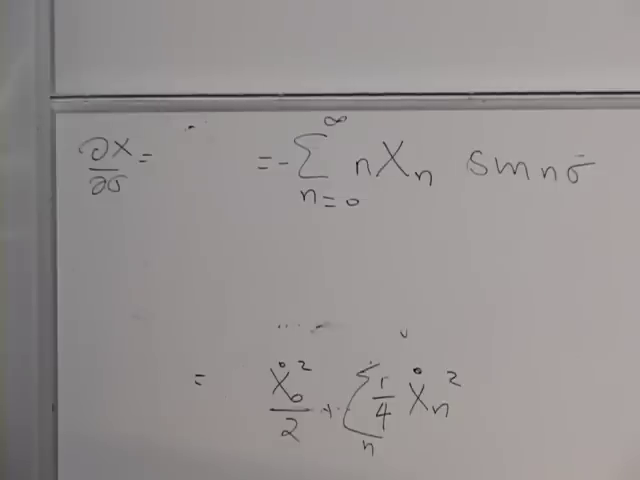
\includegraphics[width=0.68\textwidth]{lecture_02_figure_06.png}
  \caption{Энергия осциллятора, записанная так, что коэффициент при \(q^2\) сразу определяет \(\omega^2\).}
  \lectureframe{00:24:00}
  \label{fig:l02-oscillator-board}
\end{figure}

Классически \(\omega=\sqrt{\kappa/m}\); перенормировка координаты привела к тому, что \(m=1\). В квантовом случае,

\begin{equation}
  E_Q=\hbar\omega\left(Q+\frac12\right),
  \qquad Q=0,1,2,\ldots .
  \label{eq:l02-oscillator-spectrum}
\end{equation}

При обсуждении расстояний между уровнями можно вычесть общий член энергии основного состояния и сказать, что каждый квант стоит \(\hbar\omega\). В вычислении для струны мы сначала поступим именно так и отложим полную энергию нулевых колебаний.

\begin{classroomqa}
\audiencequestion{Как из формулы для энергии определяется частота осциллятора?\lecturetimestamp{00:23:21}}
\lecturerresponse{До перенормировки она равна \(\omega=\sqrt{\kappa/m}\). При единичной массе потенциальный член имеет вид \(\frac12\omega^2q^2\), так что его квадратичный коэффициент есть квадрат частоты.}
\end{classroomqa}

\section{Что делает составную систему частицей?}

Струна протяжённа и будет моделироваться множеством связанных частей. В каком смысле одно из её квантовых состояний тем не менее может быть частицей? Точечность не может быть решающим критерием. Протоны и нейтроны составны. Электроны и фотоны сопровождаются квантово-полевым облаком, хотя никакой внутренней подструктуры у них обнаружить не удалось. Классическая геометрическая точка, не окружённая ничем, — неподходящий образ квантового возбуждения.

Недостаточно и массы вместе с положением центра масс. И герметически закрытый ящик с газом, и чашка кофе обладают и тем и другим. Мы обычно не называем ни то ни другое частицей. Критерий неделимости тоже не годится, потому что протон делим, а спин не отличает микроскопические частицы от макроскопических тел.

Полезный критерий — спектральная изолированность. Отложим энергию покоя по вертикальной оси и спросим, сколько энергии нужно, чтобы перейти в другое внутреннее состояние. У электрона нет экспериментально доступной башни электронных возбуждений непосредственно над ним. У протона резонансы есть, но первые из них требуют нескольких сотен МэВ, то есть существенной доли массы протона. Эти состояния достаточно разделены, чтобы их можно было различать по отдельности.

Чашка кофе — противоположный случай. Можно сообщить сколь угодно малую энергию длинноволновой звуковой моде, слегка сдвинуть молекулу или породить фонон. В крошечном интервале упаковано чрезвычайно много состояний. В лабораторных масштабах они образуют континуум. Это и есть практическое различие между частицей и \emph{кашей}.

\begin{figure}[H]
  \centering
  \includegraphics[width=0.58\textwidth]{lecture_02_figure_07.png}
  \caption{Вертикальная ось энергии на доске при сравнении изолированного уровня частицы с плотными возбуждениями обычного вещества.}
  \lectureframe{00:31:10}
  \label{fig:l02-spectrum-board}
\end{figure}

\begin{figure}[H]
  \centering
  \begin{adjustbox}{max width=\linewidth}
  \begin{tikzpicture}[>=Latex,thick]
    \begin{scope}
      \draw[->] (0,0) -- (0,4.8) node[above] {energy};
      \draw[blue!70!black,line width=1.2pt] (-1.0,0.65) -- (1.0,0.65);
      \draw[blue!70!black,line width=1.2pt] (-1.0,3.65) -- (1.0,3.65);
      \node[right] at (1.05,0.65) {ground state};
      \node[right] at (1.05,3.65) {first internal excitation};
      \draw[<->] (0.65,0.75) -- (0.65,3.55)
        node[midway,right] {large gap};
      \node at (0,-0.55) {particle-like};
    \end{scope}
    \begin{scope}[xshift=7.0cm]
      \draw[->] (0,0) -- (0,4.8) node[above] {energy};
      \foreach \y in {0.55,0.69,0.82,0.94,1.05,1.15,1.24,1.32,1.39,1.45,
        1.51,1.57,1.63,1.70,1.78,1.87,1.97,2.09,2.22,2.36,2.51,2.67,2.84,
        3.02,3.21,3.41,3.62,3.84,4.07}
        \draw[orange!85!black] (-0.95,\y) -- (0.95,\y);
      \node[right] at (1.05,2.25) {dense phonon and internal states};
      \node at (0,-0.55) {macroscopic matter};
    \end{scope}
  \end{tikzpicture}
  \end{adjustbox}
  \caption{В лекции в качестве операционального критерия частицы используется спектральная изоляция, а не буквальная точечность.}
  \label{fig:l02-particle-redraw}
\end{figure}

Этот критерий превращает философский вопрос в расчет. Квантуйте струну, найдите ее внутренние энергетические уровни и исследуйте расстояния между ними. Если первое возбужденное состояние струны лежит вблизи планковского масштаба, тогда как наблюдаемое основное состояние имеет малую массу, то зазор превышает энергии современных ускорителей более чем на 20 порядков величины. Тогда во всей доступной области струна ведет себя как элементарная частица.

\begin{classroomqa}
\audiencequestion{Является ли поведение как у частицы лишь вопросом масштаба наблюдения? Если мы увеличим масштаб достаточно сильно, перестанут ли уровни быть раздельными?\lecturetimestamp{00:33:33}}
\lecturerresponse{Увеличение масштаба может показать, что объект состоит из многих частей, но спектр от этого не исчезает. Существенно сравнение между энергетическим разрешением эксперимента и зазором до первого внутреннего возбуждения. Составной объект может оставаться частицеподобным, если этот зазор огромен.}
\end{classroomqa}

\begin{classroomqa}
\audiencequestion{Почему обычная скрипичная струна не является частицей?\lecturetimestamp{00:34:37}}
\lecturerresponse{Энергия одного колебательного кванта неизмеримо мала по сравнению с энергией покоя макроскопической струны. Поэтому в крошечный относительный интервал укладывается множество квантовых состояний. Ее следует отнести к плотной стороне спектрального сравнения, а не к изолированной.}
\end{classroomqa}

\begin{classroomqa}
\audiencequestion{Являются ли фотоны и электроны точечными частицами, если квантовые поля окружают их виртуальными флуктуациями?\lecturetimestamp{00:35:40}}
\lecturerresponse{Классическое слово \emph{точка} здесь берет на себя слишком многое. Физические электрон и фотон — это одетые возбуждения поля, однако эксперименты не обнаружили ни у одного из них ни внутренней структуры из составляющих, ни конечного формфактора. Для данного рассуждения существенно то, что ни у одного из них нет плотной башни почти вырожденных внутренних состояний.\editorialnote{В лекции аномальный магнитный момент электрона связывается с измеримой квантовой размытостью. В современной терминологии аномальный момент — это эффект радиационного одевания, а не свидетельство экспериментально разрешимого конечного радиуса электрона. Под точечностью обычно понимают, что вплоть до проверенного масштаба не обнаружено ни внутренней подструктуры, ни формфактора.}}
\end{classroomqa}

\begin{classroomqa}
\audiencequestion{Зависит ли размер фотона от его частоты?\lecturetimestamp{00:36:49}}
\lecturerresponse{Его длина волны, конечно, зависит. Это не то же самое, что собственный размер, связанный с внутренними составляющими. Изменение частоты меняет волновой пакет и длину волны, а не разрешаемый внутренний радиус фотона.}
\end{classroomqa}

\section{Точная поперечная механика при большом импульсе}

Теперь вернемся к релятивистской трудности. Быстро вращающуюся палочку нельзя рассматривать нерелятивистски лишь потому, что ее центр масс покоится. Ее концы по-прежнему движутся друг относительно друга релятивистски. Нерелятивистское приближение оказывается неприменимым из-за внутреннего относительного движения.

Однако существует другой предел. Выберите ось \(z\) и бустируйте всю систему до очень большого положительного продольного импульса \(P_z\). Ее поперечный импульс удерживайте

\begin{equation}
  p_\perp^2=p_x^2+p_y^2
\end{equation}

конечным. Тогда поперечная проекция в пределе \(P_z\to\infty\) допускает в точности нерелятивистскую гамильтонову форму, даже если до буста внутреннее движение было релятивистским.

\begin{classroomqa}
\audiencequestion{Означает ли бесконечный импульс, что массивная система действительно достигает скорости света?\lecturetimestamp{00:40:43}}
\lecturerresponse{Ни один конечный буст не приводит к этому. Рассматривают величины, имеющие хорошо определенный предел, когда \(P_z\) становится сколь угодно большим. Это выражение обозначает предельную процедуру, а не конечное физическое состояние с \(v=c\).}
\end{classroomqa}

\begin{classroomqa}
\audiencequestion{Какую ось нужно выбрать, и что если объект вращается вокруг этой оси или поперек нее?\lecturetimestamp{00:41:14}}
\lecturerresponse{Можно выбрать любую ось и бустировать вдоль нее всю систему. В явном виде в механике остается проекция на перпендикулярную плоскость. Вращающийся стержень может выглядеть укороченным или заметать эту плоскость, но его поперечная проекция имеет нерелятивистскую форму.}
\end{classroomqa}

У струн есть дополнительное свойство, которое делает это представление необычайно мощным. В калибровке светового фронта их продольные внутренние координаты не являются независимыми осцилляторами. Связи определяют их через поперечное движение. Поэтому, зная поперечное движение струны, можно восстановить физические степени свободы.

\begin{classroomqa}
\audiencequestion{Означает ли отсутствие независимой продольной координаты, что струна просто заключена в тонкий слой?\lecturetimestamp{00:42:26}}
\lecturerresponse{Лоренцево сокращение действительно делает ее продольный размер малым в бустированной системе отсчета, но утверждение сильнее. Любое оставшееся продольное движение определяется через поперечное движение связями; его нельзя задавать независимо.}
\end{classroomqa}

\begin{classroomqa}
\audiencequestion{Связано ли это сведение к поперечным данным с голографическим принципом?\lecturetimestamp{00:43:12}}
\lecturerresponse{Это тесно связано с линией рассуждений, которая привела к голографическим идеям, хотя развитие этой связи увело бы нас от нынешнего расчета. Здесь это служит лишь обоснованием работы с поперечной струной.}
\end{classroomqa}

\subsection{Вычитание бустового вклада и перемасштабирование времени}

Пусть \(M\) — инвариантная масса полной системы, включая массы составляющих, кинетическую энергию и энергию связи. В единицах \(c=1\),

\begin{equation}
  E=\sqrt{P_z^2+p_\perp^2+M^2}.
  \label{eq:l02-relativistic-energy}
\end{equation}

При \(P_z\), значительно большем, чем \(p_\perp\) и \(M\),

\begin{equation}
  E
  =
  P_z+\frac{p_\perp^2+M^2}{2P_z}
  +O(P_z^{-3}).
  \label{eq:l02-large-pz}
\end{equation}

\begin{figure}[H]
  \centering
  \includegraphics[width=0.76\textwidth]{lecture_02_figure_08.png}
  \caption{Полное разложение при большом \(P_z\) с сохранением поперечного импульса и инвариантной массы.}
  \lectureframe{00:47:30}
  \label{fig:l02-large-pz-board}
\end{figure}

Ведущий член велик, но не несет никакой информации о внутреннем состоянии. В процессе, сохраняющем \(P_z\), например когда бустированный атом переходит между внутренними уровнями, не изменяя своего полного продольного импульса, этот член сокращается во всех разностях энергий. Поэтому мы изучаем

\begin{equation}
  E-P_z=\frac{p_\perp^2+M^2}{2P_z}+O(P_z^{-3}).
  \label{eq:l02-residual-energy}
\end{equation}

Знаменатель имеет физический смысл. Поскольку гамильтониан порождает эволюцию во времени, малая остаточная энергия означает, что внутренняя эволюция в лабораторном времени выглядит медленной. Это и есть замедление времени. Чтобы сохранить внутреннее движение, введем перемасштабированный параметр эволюции \(\tau\) или, что эквивалентно, умножим остаточный гамильтониан на \(P_z\):

\begin{equation}
  H_\perp
  \equiv
  \lim_{P_z\to\infty}P_z(E-P_z)
  =
  \frac12p_\perp^2+\frac12M^2.
  \label{eq:l02-transverse-hamiltonian}
\end{equation}

\begin{figure}[H]
  \centering
  \begin{minipage}[t]{0.48\textwidth}
    \centering
    \includegraphics[width=\textwidth]{lecture_02_figure_09.png}
    \par\smallskip\footnotesize (a) \(H=i\partial_t\) и замедленная внутренняя эволюция.
  \end{minipage}\hfill
  \begin{minipage}[t]{0.48\textwidth}
    \centering
    \includegraphics[width=\textwidth]{lecture_02_figure_10.png}
    \par\smallskip\footnotesize (b) Конечный поперечный гамильтониан после перемасштабирования времени.
  \end{minipage}
  \caption{От остаточной энергии, уменьшенной вследствие замедления времени, к конечному двумерному гамильтониану.}
  \lectureframe{00:49:20 and 00:52:40}
  \label{fig:l02-lightfront-board}
\end{figure}

Это в точности форма частицы единичной массы, движущейся в двух измерениях: кинетическая энергия \(p_\perp^2/2\) плюс внутренняя энергия \(M^2/2\). Необычность здесь в том, что фигурирует квадрат. В этом описании величина, играющая роль энергии покоя или энергии связи, пропорциональна квадрату инвариантной массы.\editorialnote{В стандартных переменных светового фронта \(P^\pm=(E\pm P_z)/\sqrt2\) точное массово-оболочечное соотношение имеет вид \(2P^+P^-=p_\perp^2+M^2\). Уравнение \eqref{eq:l02-transverse-hamiltonian} представляет собой используемую в лекции при большом \(P_z\) нормировку того же инвариантного соотношения.}

\begin{classroomqa}
\audiencequestion{Куда делись продольные импульсы отдельных частей составной системы?\lecturetimestamp{00:51:30}}
\lecturerresponse{Для общего составного объекта нужно учитывать доли полного \(P_z\), которые несут его составляющие. Формула выше использует полный импульс центра масс. Теория струн особенна тем, что ее связи определяют относительное продольное движение через поперечные степени свободы, так что добавлять независимый продольный осциллятор не требуется.}
\end{classroomqa}

\section{Дискретная открытая струна}

Бустированная струна теперь в явном виде движется только в поперечной плоскости. Обозначим ее две координаты \(X\) и \(Y\) и сначала аппроксимируем ее \(N\) материальными точками, соединенными \(N-1\) пружинами. Если \(\mu\) — аналог массы каждой точки, а \(k\) — жесткость пружины между ближайшими соседями, то энергия равна

\begin{equation}
  E_N
  =
  \sum_i
  \left[
    \frac{\mu}{2}
    \left(\dot X_i^2+\dot Y_i^2\right)
    +
    \frac{k}{2}
    \left((\Delta X_i)^2+(\Delta Y_i)^2\right)
  \right].
  \label{eq:l02-discrete-energy}
\end{equation}

Каждому члену с \(X\) соответствует идентичный член с \(Y\), потому что в поперечной плоскости есть два направления. Индекс \(i\) нумерует точку вдоль цепочки; это не пространственная координата.

\begin{figure}[H]
  \centering
  \begin{minipage}[t]{0.48\textwidth}
    \centering
    \includegraphics[width=\textwidth]{lecture_02_figure_11.png}
    \par\smallskip\footnotesize (a) Цепочка бусин и её дискретная энергия.
  \end{minipage}\hfill
  \begin{minipage}[t]{0.48\textwidth}
    \centering
    \includegraphics[width=\textwidth]{lecture_02_figure_12.png}
    \par\smallskip\footnotesize (b) Масштабирование \(\mu\) и
    \(k\) при больших \(N\).
  \end{minipage}
  \caption{Регуляризованная открытая струна до взятия предела континуума.}
  \lectureframe{00:57:42 and 01:02:40}
  \label{fig:l02-chain-board}
\end{figure}

\begin{figure}[H]
  \centering
  \begin{adjustbox}{max width=\linewidth}
  \begin{tikzpicture}[>=Latex,thick]
    \foreach \i in {0,...,8} {
      \coordinate (p\i) at ({1.05*\i},{0.30*sin(55*\i)});
      \filldraw[white] (p\i) circle (0.10);
      \draw (p\i) circle (0.10);
    }
    \foreach \i in {0,...,7} {
      \pgfmathtruncatemacro{\j}{\i+1}
      \draw[decorate,decoration={zigzag,segment length=4pt,amplitude=2pt}]
        (p\i) -- (p\j);
    }
    \node[above=0.35cm of p0] {\(i=0\)};
    \node[above=0.35cm of p8] {\(i=N-1\)};
    \draw[<->] (0,-1.15) -- (8.4,-1.15)
      node[midway,below] {\(0\leq\sigma\leq\pi\)};
    \node at (4.2,1.25)
      {\(\mu=1/N,\quad k=N/\pi^2,\quad\Delta\sigma=\pi/N\)};
  \end{tikzpicture}
  \end{adjustbox}
  \caption{Наглядная картина регулятора. По мере измельчения цепочки точки становятся легче, а микроскопические пружины — жёстче.}
  \label{fig:l02-chain-redraw}
\end{figure}

Параметр \(\sigma\) задаёт положение вдоль цепочки. Выбор
\(0\leq\sigma\leq\pi\) — это соглашение, а не измерение физической длины.
Это напоминает нам, что у струны есть два конца. Позже замкнутая струна будет
параметризоваться периодически на \(0\leq\sigma<2\pi\).

В пределе континуума коллективная механика должна оставаться конечной. При фиксированной массе бусины полная аналоговая масса расходилась бы, поэтому выберем

\begin{equation}
  \mu=\frac{1}{N}.
  \label{eq:l02-mu-scaling}
\end{equation}

Тогда \(N\mu=1\). Это не релятивистская масса покоя \(M\); это коэффициент
инерции в поперечной аналоговой модели.

Пружины, соединённые последовательно, становятся мягче по мере увеличения их
числа. Чтобы сохранить конечную жёсткость всей цепочки, каждая микроскопическая
пружина должна становиться жёстче:

\begin{equation}
  k=\frac{N}{\pi^2}
  =\frac{1}{\pi\,\Delta\sigma}.
  \label{eq:l02-k-scaling}
\end{equation}

Существенно только \(k\propto N\). Множитель \(\pi^2\) — это нормировка,
выбранная так, чтобы убрать лишние множители \(\pi\) из формул континуума.

\begin{classroomqa}
\audiencequestion{Является ли \(\mu\) физической массой покоя каждой точки струны?\lecturetimestamp{01:10:34}}
\lecturerresponse{Нет. Это нерелятивистская аналоговая масса, появляющаяся в
поперечной цепочке. Называть её \(M\) значило бы спутать её с инвариантной массой
покоя всего релятивистского состояния струны. Её единственная нынешняя роль —
обеспечить правильную инерцию в пределе континуума.}
\end{classroomqa}

\section{Континуальная волновая система}

Применим правила, подготовленные в начале. Поскольку
\(1/N=\Delta\sigma/\pi\),

\begin{align}
  \sum_i\frac{\mu}{2}\dot X_i^2
  &=
  \frac{1}{2\pi}
  \sum_i\dot X_i^2\,\Delta\sigma
  \longrightarrow
  \frac{1}{2\pi}
  \int_0^\pi
  \left(\partial_\tau X\right)^2d\sigma ,
  \label{eq:l02-kinetic-limit}\\
  \sum_i\frac{k}{2}(\Delta X_i)^2
  &\longrightarrow
  \frac{1}{2\pi}
  \int_0^\pi
  \left(\partial_\sigma X\right)^2d\sigma .
  \label{eq:l02-potential-limit}
\end{align}

Для второй строки используем
\(\Delta X_i=\partial_\sigma X\,\Delta\sigma\) вместе с
\(k=1/(\pi\Delta\sigma)\). То же вычисление применимо и к \(Y\).

\begin{figure}[H]
  \centering
  \begin{minipage}[t]{0.48\textwidth}
    \centering
    \includegraphics[width=\textwidth]{lecture_02_figure_13.png}
    \par\smallskip\footnotesize (a) Замены суммы на интеграл и
    разности на производную.
  \end{minipage}\hfill
  \begin{minipage}[t]{0.48\textwidth}
    \centering
    \includegraphics[width=\textwidth]{lecture_02_figure_14.png}
    \par\smallskip\footnotesize (b) Полная энергия в пределе континуума.
  \end{minipage}
  \caption{Переход дискретной цепочки в поле на интервале \(\sigma\).}
  \lectureframe{01:05:40 and 01:07:00}
  \label{fig:l02-continuum-board}
\end{figure}

В результате энергия и лагранжиан имеют вид

\begin{align}
  E
  &=
  \frac{1}{2\pi}
  \int_0^\pi d\sigma\,
  \left[
    (\partial_\tau X)^2+(\partial_\tau Y)^2\right.\notag\\[-0.25em]
  &\hspace{6.5em}\left.
    +(\partial_\sigma X)^2+(\partial_\sigma Y)^2
  \right],
  \label{eq:l02-continuum-energy}\\
  L
  &=
  \frac{1}{2\pi}
  \int_0^\pi d\sigma\,
  \left[
    (\partial_\tau X)^2+(\partial_\tau Y)^2\right.\notag\\[-0.25em]
  &\hspace{6.5em}\left.
    -(\partial_\sigma X)^2-(\partial_\sigma Y)^2
  \right].
  \label{eq:l02-continuum-lagrangian}
\end{align}

\begin{figure}[H]
  \centering
  \includegraphics[width=0.78\textwidth]{lecture_02_figure_15.png}
  \caption{Континуальный лагранжиан, в котором кинетический член и член растяжения
  входят с противоположными знаками.}
  \lectureframe{01:08:48}
  \label{fig:l02-lagrangian-board}
\end{figure}

Если переобозначить \(\sigma\) как обычную пространственную координату, а \(X\) как
поле \(\phi\), то это энергия и лагранжиан одномерного волнового
поля. Варьирование \eqref{eq:l02-continuum-lagrangian} даёт

\begin{equation}
  \left(\partial_\tau^2-\partial_\sigma^2\right)X=0,
  \qquad
  \left(\partial_\tau^2-\partial_\sigma^2\right)Y=0.
  \label{eq:l02-wave-equation}
\end{equation}

В непосредственном рассуждении ничто не требует от нас решать эти уравнения
напрямую. Полезная картина проста: волны распространяются влево и вправо вдоль
струны и отражаются на концах. При отражении Дирихле знак смещения
меняется на противоположный; при отражении Неймана он сохраняется.

\begin{classroomqa}
\audiencequestion{Что именно представляет собой временная переменная
\(\tau\)?\lecturetimestamp{01:08:54}}
\lecturerresponse{Это перенормированное время, используемое для отслеживания внутреннего движения
в описании при больших \(P_z\). Часы, подвергнутые тому же бусту, идут медленнее
относительно лабораторного времени; \(\tau\) устраняет это замедление, так
что внутренние колебания сохраняют конечную частоту. Для этой поперечной
механики его можно просто считать временем.\editorialnote{Лекция неформально
называет \(\tau\) собственным временем. Для протяжённой струны точным
параметром эволюции по световому фронту служит калибровочно фиксированное
перенормированное время, а не единое инвариантное собственное время,
общее для каждой точки. Подразумевавшийся аргумент о замедлении времени
при этом не меняется.}}
\end{classroomqa}

Когда центр масс покоится в поперечной плоскости, внутренняя
часть \eqref{eq:l02-continuum-energy} в нормировке
\eqref{eq:l02-transverse-hamiltonian} пропорциональна \(M^2\). Именно поэтому
квантование этой на вид обычной волновой системы обнаружит релятивистский
спектр масс.

\begin{classroomqa}
\audiencequestion{Есть ли у \(P_z(E-P_z)\)
название?\lecturetimestamp{01:11:00}}
\lecturerresponse{Его обычно называют энергией светового конуса или светового фронта.
Термин световой фронт точнее описывает нулевую плоскость, используемую как
поверхность эволюции; традиционная терминология не важна для вычисления.}
\end{classroomqa}

\begin{classroomqa}
\audiencequestion{Относится ли слово конус к обычному световому
конусу пространства-времени и ввёл ли эту терминологию Dirac?\lecturetimestamp{01:11:17}}
\lecturerresponse{Построение с нулевыми координатами можно изобразить с осями под
45 градусами, но поверхность эволюции здесь — световой фронт, а не
весь расширяющийся конус. Dirac развил родственные формы релятивистской
динамики; исторический вопрос о названии оставили открытым, и на уравнения
это не влияет.}
\end{classroomqa}

\section{Почему свободный конец подчиняется условию Неймана}

Теперь граничное условие на конце можно вывести, а не постулировать. Закон Ньютона
здесь правомерен, потому что бустированная поперечная механика имеет в точности
нерелятивистскую форму. На внутреннюю материальную точку тянут пружины с обеих
сторон. На последнюю точку действует только пружина, соединяющая её с
соседней.

\begin{classroomqa}
\audiencequestion{Почему, обсуждая релятивистскую струну, мы вправе пользоваться законом
Ньютона?\lecturetimestamp{01:14:52}}
\lecturerresponse{Мы не применяем ньютонову механику к полному
небустированному движению в пространстве-времени. Мы применяем её к поперечным
переменным в описании при бесконечном импульсе, гамильтониан которого имеет в
точности нерелятивистскую форму.}
\end{classroomqa}

На правом конце закон Гука даёт, с точностью до выбора направления,

\begin{equation}
  F_{\mathrm{end}}
  =
  -k\,\Delta X
  =
  -\frac{1}{\pi\Delta\sigma}
   \left(\partial_\sigma X\,\Delta\sigma\right)
  =
  -\frac{1}{\pi}\partial_\sigma X .
  \label{eq:l02-endpoint-force}
\end{equation}

\begin{figure}[H]
  \centering
  \begin{minipage}[t]{0.48\textwidth}
    \centering
    \includegraphics[width=\textwidth]{lecture_02_figure_16.png}
    \par\smallskip\footnotesize (a) Сила на конце пропорциональна локальному
    наклону.
  \end{minipage}\hfill
  \begin{minipage}[t]{0.48\textwidth}
    \centering
    \includegraphics[width=\textwidth]{lecture_02_figure_17.png}
    \par\smallskip\footnotesize (b) Условие конечности ускорения.
  \end{minipage}
  \caption{Вывод граничного условия для свободного конца из закона Ньютона.}
  \lectureframe{01:18:20 and 01:20:10}
  \label{fig:l02-neumann-board}
\end{figure}

Уравнение Ньютона для последней точки имеет вид

\begin{equation}
  \mu\,\partial_\tau^2X=F_{\mathrm{end}},
  \qquad
  \mu=\frac1N=\frac{\Delta\sigma}{\pi}.
  \label{eq:l02-endpoint-newton}
\end{equation}

Комбинируя \eqref{eq:l02-endpoint-force} и
\eqref{eq:l02-endpoint-newton},

\begin{equation}
  \partial_\sigma X
  =
  -\Delta\sigma\,\partial_\tau^2X
  \quad\text{at the right endpoint},
  \label{eq:l02-endpoint-scaling}
\end{equation}

причём на левом конце знак силы меняется на противоположный. Если бы
\(\partial_\sigma X\) стремилась к ненулевой константе при
\(\Delta\sigma\to0\), ускорение конца расходилось бы как \(N\).
Поэтому разумный предел континуума с конечным ускорением требует

\begin{equation}
  \left.\partial_\sigma X\right|_{0,\pi}=0,
  \qquad
  \left.\partial_\sigma Y\right|_{0,\pi}=0.
  \label{eq:l02-open-neumann}
\end{equation}

\begin{figure}[H]
  \centering
  \begin{adjustbox}{max width=\linewidth}
  \begin{tikzpicture}[>=Latex,thick,scale=1.0]
    \coordinate (a) at (0,0);
    \coordinate (b) at (4.5,0.75);
    \filldraw[white] (a) circle (0.12);
    \draw (a) circle (0.12);
    \filldraw[white] (b) circle (0.12);
    \draw (b) circle (0.12);
    \draw[decorate,decoration={zigzag,segment length=6pt,amplitude=3pt}]
      (a) -- (b);
    \draw[dashed] (a) -- (0,-1.2);
    \draw[dashed] (b) -- (4.5,-1.2);
    \draw[<->] (4.85,0) -- (4.85,0.75)
      node[midway,right] {\(\Delta X\)};
    \draw[->,red!70!black] (b) -- (5.75,0.95)
      node[right] {\(F_{\rm end}=-k\Delta X\)};
    \node[below] at (0,-1.2) {\(N-1\)};
    \node[below] at (4.5,-1.2) {\(N\)};
    \node at (2.5,-2.0)
      {\(\mu\ddot X=-k\Delta X
      \ \Longrightarrow\
      \partial_\sigma X=-\Delta\sigma\,\ddot X\to0\)};
  \end{tikzpicture}
  \end{adjustbox}
  \caption{В пределе регулятора масса последней точки стремится к нулю. Конечное
  ускорение возможно только тогда, когда наклон на конце обращается в нуль.}
  \label{fig:l02-neumann-redraw}
\end{figure}

Тот же аргумент на обоих концах и в обоих поперечных направлениях даёт
условия Неймана для свободной открытой струны.

\section{Нормальные моды открытой струны}

Теперь у нас есть полная классическая система: лагранжиан и его граничные
условия. После разложения в ряд Фурье квантование становится простым. Поскольку
на концах выполняются условия Неймана,

\begin{align}
  X(\sigma,\tau)
  &=
  \sum_{n=0}^{\infty}X_n(\tau)\cos(n\sigma),
  \label{eq:l02-X-expansion}\\
  Y(\sigma,\tau)
  &=
  \sum_{n=0}^{\infty}Y_n(\tau)\cos(n\sigma).
  \label{eq:l02-Y-expansion}
\end{align}

Косинусы содержат всю зависимость от \(\sigma\). Коэффициенты содержат всю
зависимость от времени; струна колеблется, потому что меняются \(X_n(\tau)\) и \(Y_n(\tau)\).

\begin{figure}[H]
  \centering
  \includegraphics[width=0.78\textwidth]{lecture_02_figure_18.png}
  \caption{Разложение по модам Неймана, помещённое рядом с правилом ортогональности,
  которое сведёт двойные суммы.}
  \lectureframe{01:21:45}
  \label{fig:l02-mode-expansion-board}
\end{figure}

\subsection{Кинетический член и нулевая мода}

Дифференцирование по времени даёт

\begin{equation}
  \partial_\tau X
  =
  \sum_{n=0}^{\infty}\dot X_n(\tau)\cos(n\sigma).
  \label{eq:l02-time-mode}
\end{equation}

После возведения в квадрат получается двойная сумма по \(n\) и \(m\), но \eqref{eq:l02-cos-orthogonality} устраняет каждое слагаемое с \(n\neq m\).
Рассматривая постоянную моду отдельно,

\begin{equation}
  \frac{1}{2\pi}\int_0^\pi
  (\partial_\tau X)^2\,d\sigma
  =
  \frac12\dot X_0^{\,2}
  +
  \frac14\sum_{n=1}^{\infty}\dot X_n^{\,2}.
  \label{eq:l02-mode-kinetic}
\end{equation}

\begin{figure}[H]
  \centering
  \includegraphics[width=0.76\textwidth]{lecture_02_figure_19.png}
  \caption{Интеграл ортогональности, сводящий двойную сумму в кинетическом члене к нулевой моде и диагональной сумме.}
  \lectureframe{01:29:10}
  \label{fig:l02-mode-kinetic-board}
\end{figure}

Постоянный коэффициент — это среднее положение,

\begin{equation}
  X_0(\tau)=\frac1\pi\int_0^\pi X(\sigma,\tau)\,d\sigma ,
  \label{eq:l02-center-of-mass}
\end{equation}

и аналогично для \(Y_0\). При равномерной массовой плотности в этой аналогии это координаты центра масс. У них есть кинетическая энергия, но нет возвращающей силы:
вся струна может свободно двигаться по поперечной плоскости.

\subsection{Член растяжения и частоты осцилляторов}

Пространственное дифференцирование даёт

\begin{equation}
  \partial_\sigma X
  =
  -\sum_{n=1}^{\infty}nX_n(\tau)\sin(n\sigma).
  \label{eq:l02-spatial-mode}
\end{equation}

Нулевая мода исчезает, потому что однородная трансляция не растягивает струну. Используя ортогональность синусов,

\begin{equation}
  \frac{1}{2\pi}\int_0^\pi
  (\partial_\sigma X)^2\,d\sigma
  =
  \frac14\sum_{n=1}^{\infty}n^2X_n^{\,2}.
  \label{eq:l02-mode-potential}
\end{equation}

\begin{figure}[H]
  \centering
  \includegraphics[width=0.76\textwidth]{lecture_02_figure_20.png}
  \caption{Дифференцирование косинусного ряда даёт двойную сумму по синусам; ортогональность снова приводит к \(n=m\).}
  \lectureframe{01:31:40}
  \label{fig:l02-mode-potential-board}
\end{figure}

Следовательно, лагранжиан \(X\)-сектора имеет вид

\begin{equation}
  L_X
  =
  \frac12\dot X_0^{\,2}
  +
  \frac14\sum_{n=1}^{\infty}
  \left(
    \dot X_n^{\,2}-n^2X_n^{\,2}
  \right),
  \label{eq:l02-X-lagrangian}
\end{equation}

и с тождественным выражением для \(Y\). В соответствующей энергии перед \(n^2X_n^2\) стоит знак плюс. Каждая ненулевая мода представляет собой независимый гармонический осциллятор, и сравнение с \eqref{eq:l02-oscillator-lagrangian} даёт

\begin{equation}
  \omega_n=n,
  \qquad n=1,2,3,\ldots .
  \label{eq:l02-mode-frequency}
\end{equation}

\begin{figure}[H]
  \centering
  \includegraphics[width=0.80\textwidth]{lecture_02_figure_21.png}
  \caption{Лагранжиан развязанных осцилляторов и вывод \(\omega_n=n\), а внизу показана тождественная башня \(Y\).}
  \lectureframe{01:35:50}
  \label{fig:l02-oscillator-modes-board}
\end{figure}

Нормальные моды — это просто гармоники струны. Первая изгибается медленно, у второй частота вдвое больше, у третьей — втрое, и так далее. Именно ортогональность не даёт одной гармонике связываться с другой в свободной теории.

\begin{classroomqa}
\audiencequestion{Что произошло с осциллятором \(n=0\)?\lecturetimestamp{01:34:49}}
\lecturerresponse{У него нулевая частота, потому что это вовсе не внутренний осциллятор. Он описывает трансляцию центра масс. Никакая пружина не возвращает всю струну к некоторому предпочтительному поперечному положению, поэтому нулевая мода является координатой свободной частицы.}
\end{classroomqa}

Если отбросить кинетический член центра масс, остаётся внутренняя энергия

\begin{equation}
  E_{\mathrm{int}}
  =
  \frac14
  \sum_{n=1}^{\infty}
  \left[
    \dot X_n^{\,2}+n^2X_n^{\,2}
    +\dot Y_n^{\,2}+n^2Y_n^{\,2}
  \right].
  \label{eq:l02-internal-energy}
\end{equation}

В нормировке светового фронта эта величина пропорциональна квадрату инвариантной массы состояния струны. Таким образом, мы свели релятивистскую задачу о массе к квантовой механике двух счётных башен осцилляторов.

\section{Квантованные уровни и поведение как у частиц}

Пусть \(a_n^\dagger\) создаёт 1 квант в \(X\)-осцилляторе с частотой \(n\), а \(b_n^\dagger\) делает то же самое для \(Y\). В лекции систематическое операторное рассмотрение откладывается, но это обозначение делает подсчёт уровней наглядным. Относительно сдвига энергии основного состояния,

\begin{equation}
  \begin{aligned}
    \Delta E_{\mathrm{int}}
    &=\sum_{n=1}^{\infty}n\left(Q_n^X+Q_n^Y\right),\\
    Q_n^X,Q_n^Y&\in\{0,1,2,\ldots\}.
  \end{aligned}
  \label{eq:l02-quantized-energy}
\end{equation}

где \(\hbar=1\). Целое число \(n\) указывает, какой осциллятор возбуждён; \(Q_n\) показывает, сколько квантов в нём находится.\editorialnote{Каждый осциллятор также вносит энергию нулевых колебаний. Бесконечная сумма требует регуляризации и даёт интерсепт в формуле масс струны. В лекции здесь намеренно не указывается сдвиг основного состояния и учитываются только уровни возбуждения.}

Осцилляторный вакуум \(\ket{0}\) — это не пустое пространство-время. Это 1 открытая струна, в которой не возбуждён ни один внутренний осциллятор. У неё есть энергия, импульс и определённое место в спектре струн.

На первом уровне есть 2 состояния,

\begin{equation}
  a_1^\dagger\ket{0},
  \qquad
  b_1^\dagger\ket{0},
  \label{eq:l02-level-one}
\end{equation}

соответствующие низшей гармонике, поляризованной вдоль \(X\) или \(Y\). Линейные комбинации описывают любую поперечную поляризацию.

На втором уровне есть 5 состояний:

\begin{equation}
  (a_1^\dagger)^2\ket{0},
  \quad
  a_1^\dagger b_1^\dagger\ket{0},
  \quad
  (b_1^\dagger)^2\ket{0},
  \quad
  a_2^\dagger\ket{0},
  \quad
  b_2^\dagger\ket{0}.
  \label{eq:l02-level-two}
\end{equation}

В 3 из них используются 2 кванта первой гармоники; в 2 — 1 квант второй гармоники. Оба построения обходятся в 2 единицы.

\begin{figure}[H]
  \centering
  \includegraphics[width=0.76\textwidth]{lecture_02_figure_22.png}
  \caption{Пять состояний второго уровня, перечисляемые заново после вопроса из аудитории: 2 двойных возбуждения, 1 смешанное возбуждение и 2 возбуждения второй гармоники.}
  \lectureframe{01:44:00}
  \label{fig:l02-levels-board}
\end{figure}

\begin{figure}[H]
  \centering
  \begin{adjustbox}{max width=\linewidth}
  \begin{tikzpicture}[>=Latex,thick]
    \draw[->] (0,0) -- (0,5.1) node[above] {\(\Delta E_{\rm int}\)};
    \draw[blue!70!black] (-0.65,0.55) -- (0.65,0.55);
    \node[right] at (0.85,0.55) {\(\ket{0}\) \quad multiplicity \(1\)};
    \draw[blue!70!black] (-0.65,2.15) -- (0.65,2.15);
    \node[right] at (0.85,2.15)
      {\(a_1^\dagger\ket{0},\ b_1^\dagger\ket{0}\)
      \quad multiplicity \(2\)};
    \draw[blue!70!black] (-0.65,3.75) -- (0.65,3.75);
    \node[right,text width=8.6cm] at (0.85,3.75)
      {\((a_1^\dagger)^2\ket{0},
      a_1^\dagger b_1^\dagger\ket{0},
      (b_1^\dagger)^2\ket{0},
      a_2^\dagger\ket{0},\ b_2^\dagger\ket{0}\)
      \quad multiplicity \(5\)};
    \node[left] at (-0.75,0.55) {\(0\)};
    \node[left] at (-0.75,2.15) {\(1\)};
    \node[left] at (-0.75,3.75) {\(2\)};
  \end{tikzpicture}
  \end{adjustbox}
  \caption{Первые 3 уровня возбуждения открытой струны с двумя поперечными направлениями.}
  \label{fig:l02-levels-redraw}
\end{figure}

\begin{classroomqa}
\audiencequestion{На втором возбуждённом уровне 4 или 5 состояний?\lecturetimestamp{01:43:04}}
\lecturerresponse{Пять. Двукратное возбуждение \(X_1\), двукратное возбуждение \(Y_1\) и их однократное совместное возбуждение дают 3 состояния. Однократное возбуждение \(X_2\) или однократное возбуждение \(Y_2\) дают ещё 2. В качестве упражнения предлагается подсчитать следующие 2 уровня.}
\end{classroomqa}

Существенный вывод уже виден. Последовательные уровни разделены конечными промежутками, и каждый имеет конечную кратность. Поэтому квантованная струна подобна частице по спектральному критерию, который отличал её от кофе, газа или обычной скрипичной струны. Позже мы определим, какие состояния физически приемлемы, а какие патологии должны быть устранены.

\section{Почему взаимодействия открытых струн порождают замкнутые струны}

У открытой струны есть 2 конца. Её элементарные взаимодействия соединяют и расщепляют струны. В адронной картине можно вообразить кварк на одном конце и антикварк на другом; их аннигиляция соединяет 2 участка струны. Интересующие нас далее фундаментальные струны не обязаны допускать столь буквальную адронную интерпретацию концов, но локальное правило соединения сохраняется.

Теперь пусть 1 открытая струна флуктуирует так, что её собственные концы сближаются друг с другом. Локально конец не может знать, принадлежит ли другой конец той же струне, а не другой. Если концам вообще разрешено соединяться, они могут соединиться и здесь, образуя замкнутую петлю.

\begin{figure}[H]
  \centering
  \includegraphics[width=0.70\textwidth]{lecture_02_figure_23.png}
  \caption{Набросок на доске: открытая струна флуктуирует, пока её 2 конца не встретятся и не образуют замкнутую петлю.}
  \lectureframe{01:47:00}
  \label{fig:l02-closed-board}
\end{figure}

\begin{figure}[H]
  \centering
  \begin{adjustbox}{max width=\linewidth}
  \begin{tikzpicture}[>=Latex,thick]
    \begin{scope}
      \draw[blue!70!black]
        (0,0) .. controls (0.8,1.2) and (1.7,-1.0) .. (2.6,0.45)
        .. controls (3.4,1.55) and (4.0,0.3) .. (4.7,0.85);
      \fill (0,0) circle (0.09);
      \fill (4.7,0.85) circle (0.09);
      \node at (2.35,-1.25) {open string fluctuation};
    \end{scope}
    \draw[->,line width=1pt] (5.25,0.3) -- (6.65,0.3)
      node[midway,above] {join};
    \begin{scope}[xshift=8.1cm]
      \draw[orange!85!black]
        (0,0) .. controls (0.3,1.5) and (2.5,1.8) .. (3.1,0.3)
        .. controls (3.5,-1.1) and (0.7,-1.5) .. (0,0);
      \node at (1.55,-1.85) {closed string};
    \end{scope}
  \end{tikzpicture}
  \end{adjustbox}
  \caption{Как только соединение концов разрешено, открытая струна может замкнуться на себя.}
  \label{fig:l02-closed-redraw}
\end{figure}

Таким образом, теория может содержать замкнутые струны без открытых, но взаимодействующая теория с открытыми струнами не может последовательно обойтись без замкнутых. Эта асимметрия и является важным предсказанием. Отождествления состояний спектра будут развиты позже, но конечный пункт уже виден: безмассовые состояния открытой струны часто соответствуют калибровочным частицам, таким как фотоны, тогда как спектр замкнутой струны содержит безмассовое состояние со спином 2, гравитон. Замкнутые струны, а следовательно и гравитация, не являются необязательным украшением, как только в теории струн есть взаимодействия.